\documentclass[12pt]{article}
%\usepackage[pass,letterpaper]{geometry}              %This package needs to be enaled when dvi--->ps----->PDF
\usepackage{stmaryrd, amsfonts, mathptmx, mathtools, array, siunitx, subfigure, graphicx, listings, etoolbox, mdwlist }
\usepackage{multirow, indentfirst, cite, verbatim, keyval, textcomp, enumerate, calc, microtype, color,marvosym}

\usepackage[colorlinks,linktocpage,dvips]{hyperref}
\hypersetup{
   colorlinks   = true,                               %Colours links instead of ugly boxes
   urlcolor     = blue,                               %Colour for external hyper links
   linkcolor    = blue,                               %Colour of internal links
   citecolor    = red,                                %Colour of citations
   setpagesize  = false,
   linktocpage  = true,
}

\makeatletter
\patchcmd{\l@section}
  {\hfil}
  {\leaders\hbox{\normalfont$\m@th\mkern \@dotsep mu\hbox{.}\mkern \@dotsep mu$}\hfill}
  {}{}
\makeatother
\definecolor{anti-flashwhite}{rgb}{0.95, 0.95, 0.96}
\lstset{
backgroundcolor=\color{anti-flashwhite},
basicstyle=\small\ttfamily,
columns=flexible,
breaklines=true
}


\newcommand{\shellcmd}[1]{\\\indent\indent\texttt{\footnotesize\$ #1}\\}
\parskip 0.5em
\parindent 2em
\setlength{\textwidth}{6.0in} \setlength{\textheight}{8.8in}
\setlength{\topmargin}{0.4in} \setlength{\headheight}{0.0in}
\setlength{\headsep}{0.0in} \setlength{\oddsidemargin}{0.25in}
\setlength{\parindent}{.2in}
%\renewcommand{\baselinestretch}{1.5}
\setlength{\parindent}{2em}
\setlength{\parskip}{1em}
%%%%%%%%%%%%%%%%%%%%%%%%%%%%%%%%%%%%%%%%%%%%%%%%%%%%%%%%%%%%%%%%%%%%%%%%%%%
\title{\textbf{GETTING STARTED GUIDE FOR}\\\textbf{THEANO, TENSORFLOW, CAFFE}\\ \textbf{WITH PYCHARM}}%

\author{Data Science Program, GWU, USA \\
School of Electrical and Computer Engineering, OSU, USA\\
\vspace{1cm}\\
\Letter : martin.t.hagan@okstate.edu\\
\Letter : ajafari@gwu.edu\\
\Letter : amir.h.jafari@okstate.edu  }
%%%%%%%%%%%%%%%%%%%%%%%%%%%%%%%%%%%%%%%%%%%%%%%%%%%%%%%%%%%%%%%%%%%%%%%%%%%
\begin{document}
\begin{figure}
\centering 
\includegraphics[width=2in, height=1in]{fig/GW_logo.eps}\hfill
\centering 
\includegraphics[width=1in, height=1in]{fig/logo1.eps}\hfill
\end{figure}

%%%%%%%%%%%%%%%%%%%%%%%%%%%%%%%%%%%%%%%%%%%%%%%%%%%%%%%%%%%%%%%%%%%%%%%%%%%
\maketitle
\newpage
\tableofcontents
\newpage
\listoffigures
\newpage
%\listoftables
% \newpage
%\lstlistoflistings
% \newpage
%%%%%%%%%%%%%%%%%%%%%%%%%%%%%%%%%%%%%%%%%%%%%%%%%%%%%%%%%%%%%%%%%%%%%%%%%%%
\section{Caffe}

\begin{enumerate}
  \item To use Caffe software in Pycharm, you need to set the environments for CUDA and Pyhon path.
  \item Open up VNC server and use your password to enter the Linux station.
  \item By this time you should be able to see the Ubuntu Desktop shown in Figure \ref{fig:1}.
\suspend{enumerate}
\begin{figure}[h]
	\centerline{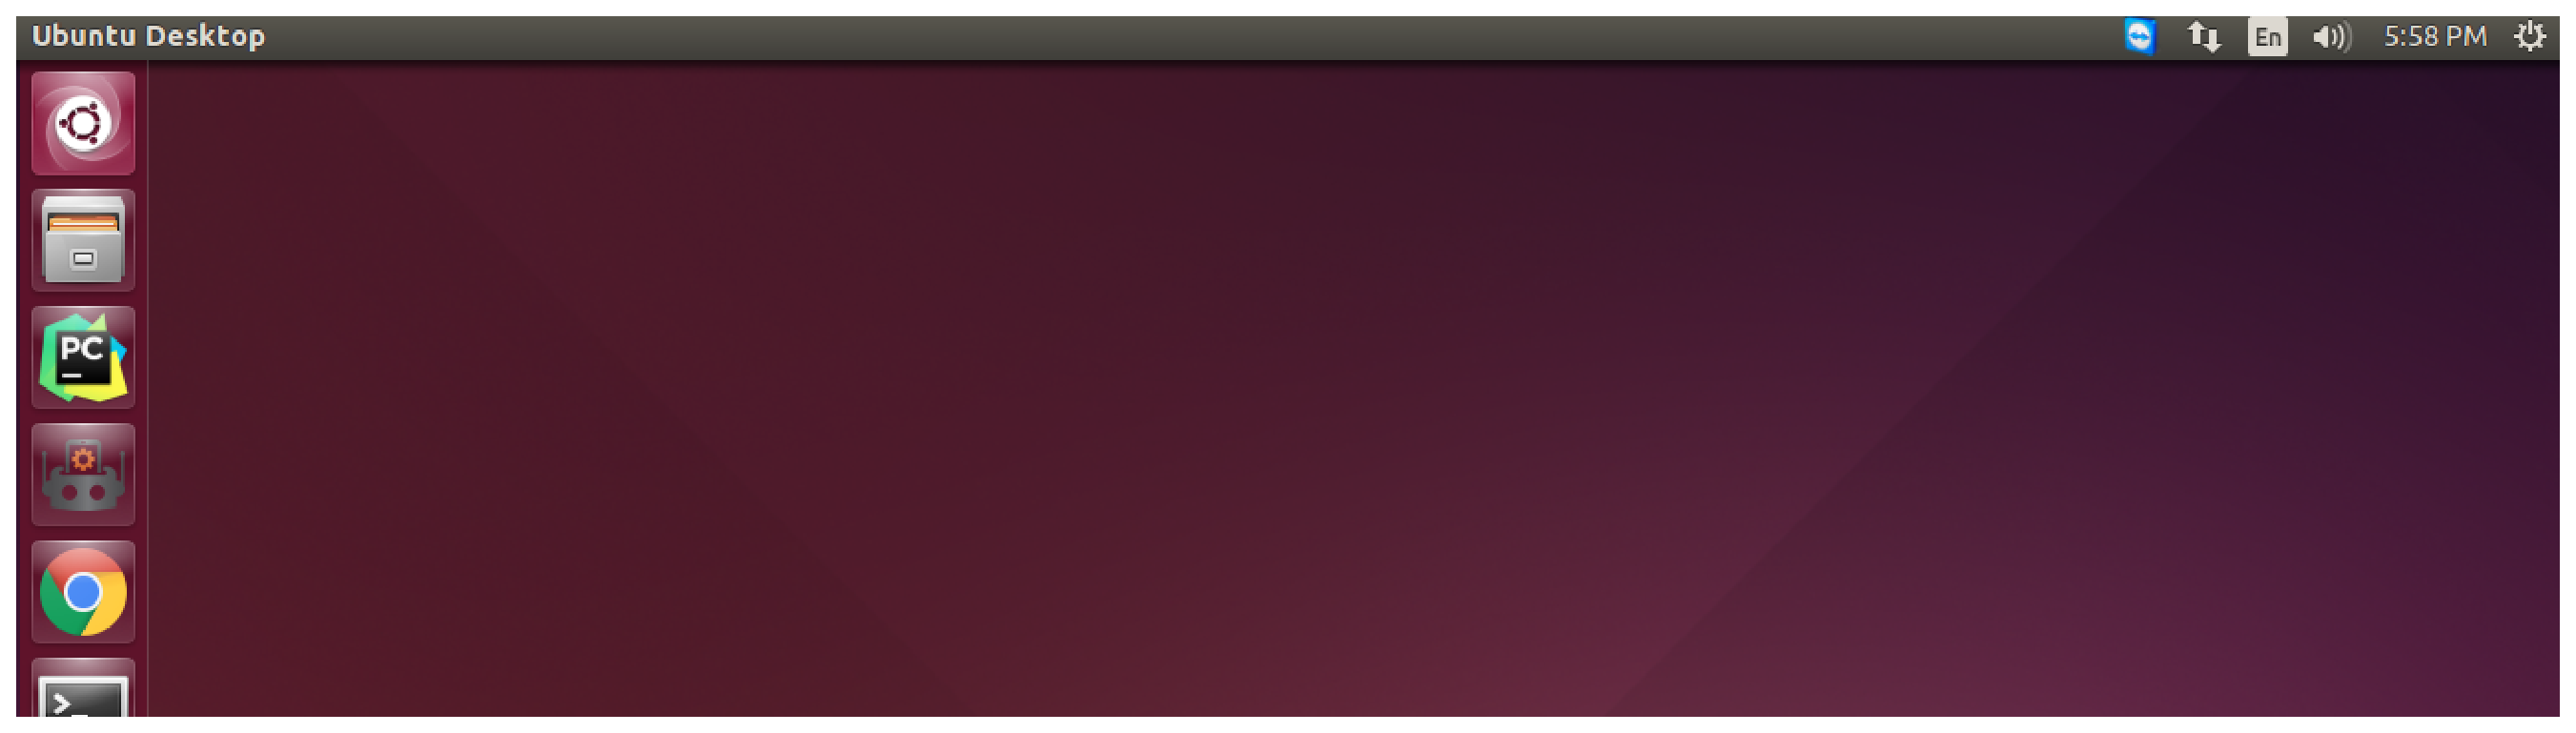
\includegraphics[width=6in, height=1.6in]{fig/1.eps}}
	\caption{Ubuntu Desktop-Caffe}
	\label{fig:1}
\end{figure}
\resume{enumerate}
  \item On the top left corner of the Ubuntu Desktop, the first icon is search box.
  \item Click on it and search the word pycharm.
  \item By this time you should be able to see the pycharm IDE and launch it by clicking on it.
  \item By this time, you should be able to see Figure \ref{fig:2}
\suspend{enumerate}
\begin{figure}[h]
	\centerline{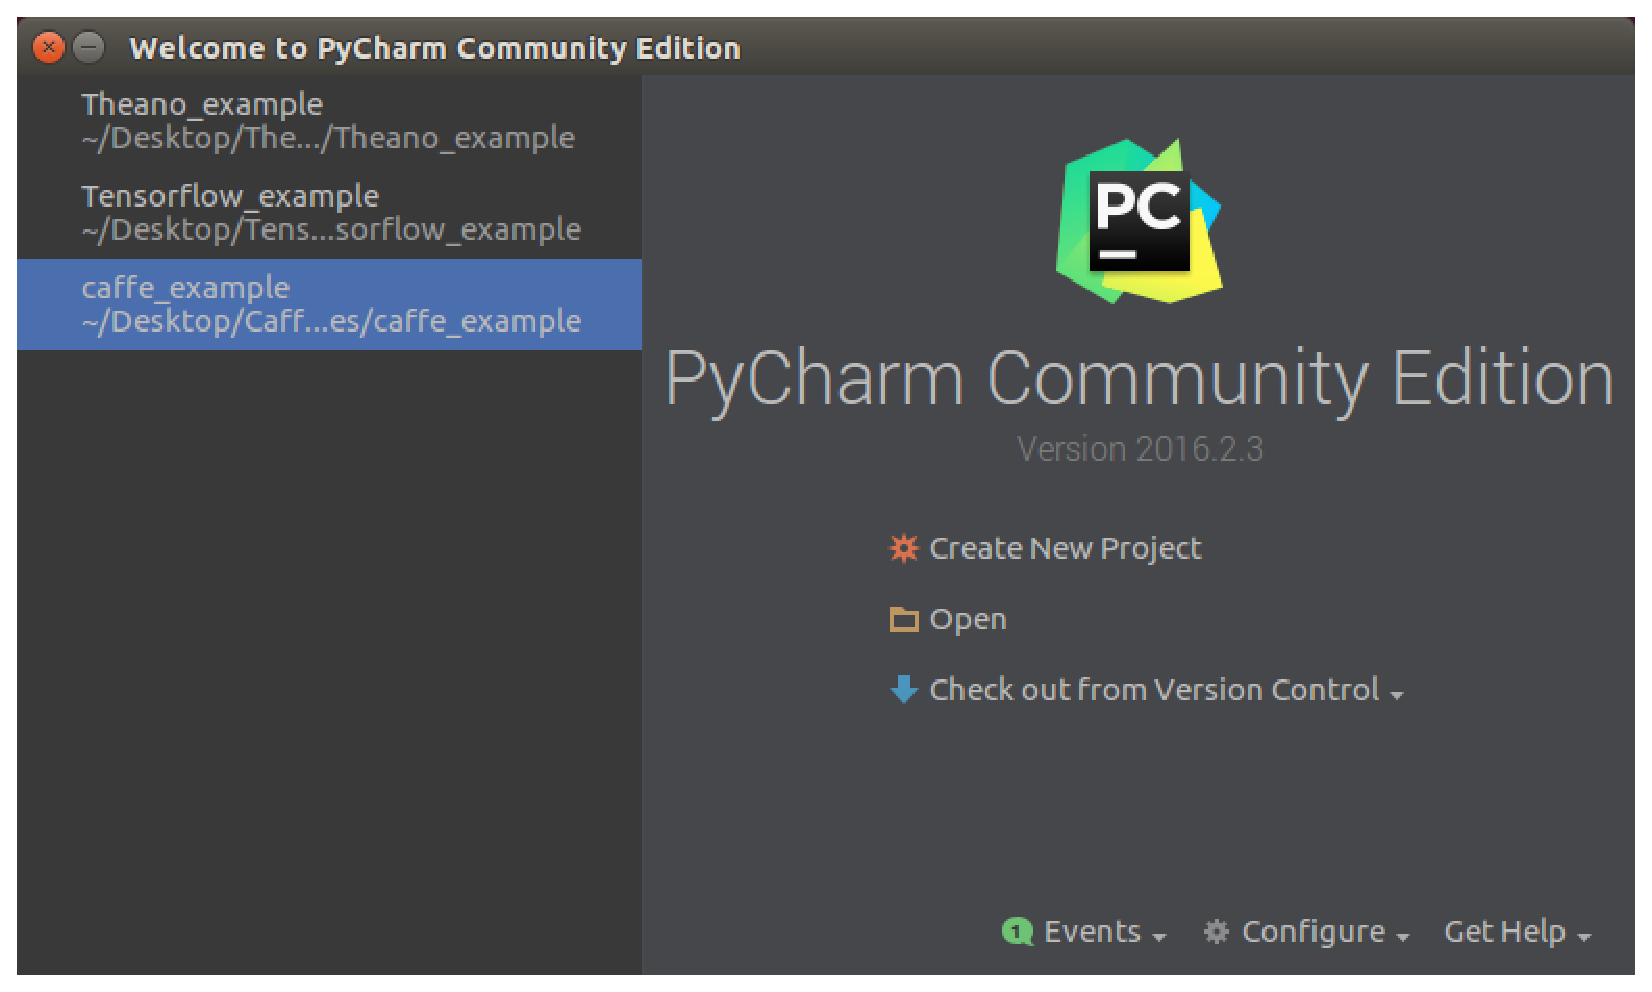
\includegraphics[width=3.5in, height=2.3in]{fig/2.eps}}
	\caption{Pycharm IDE}
	\label{fig:2}
\end{figure}
\resume{enumerate}
  \item Now, we need to create a project, click on create new project icon.
  \item It opens up a new window shown in Figure \ref{fig:3}.
\suspend{enumerate}
\begin{figure}[h]
	\centerline{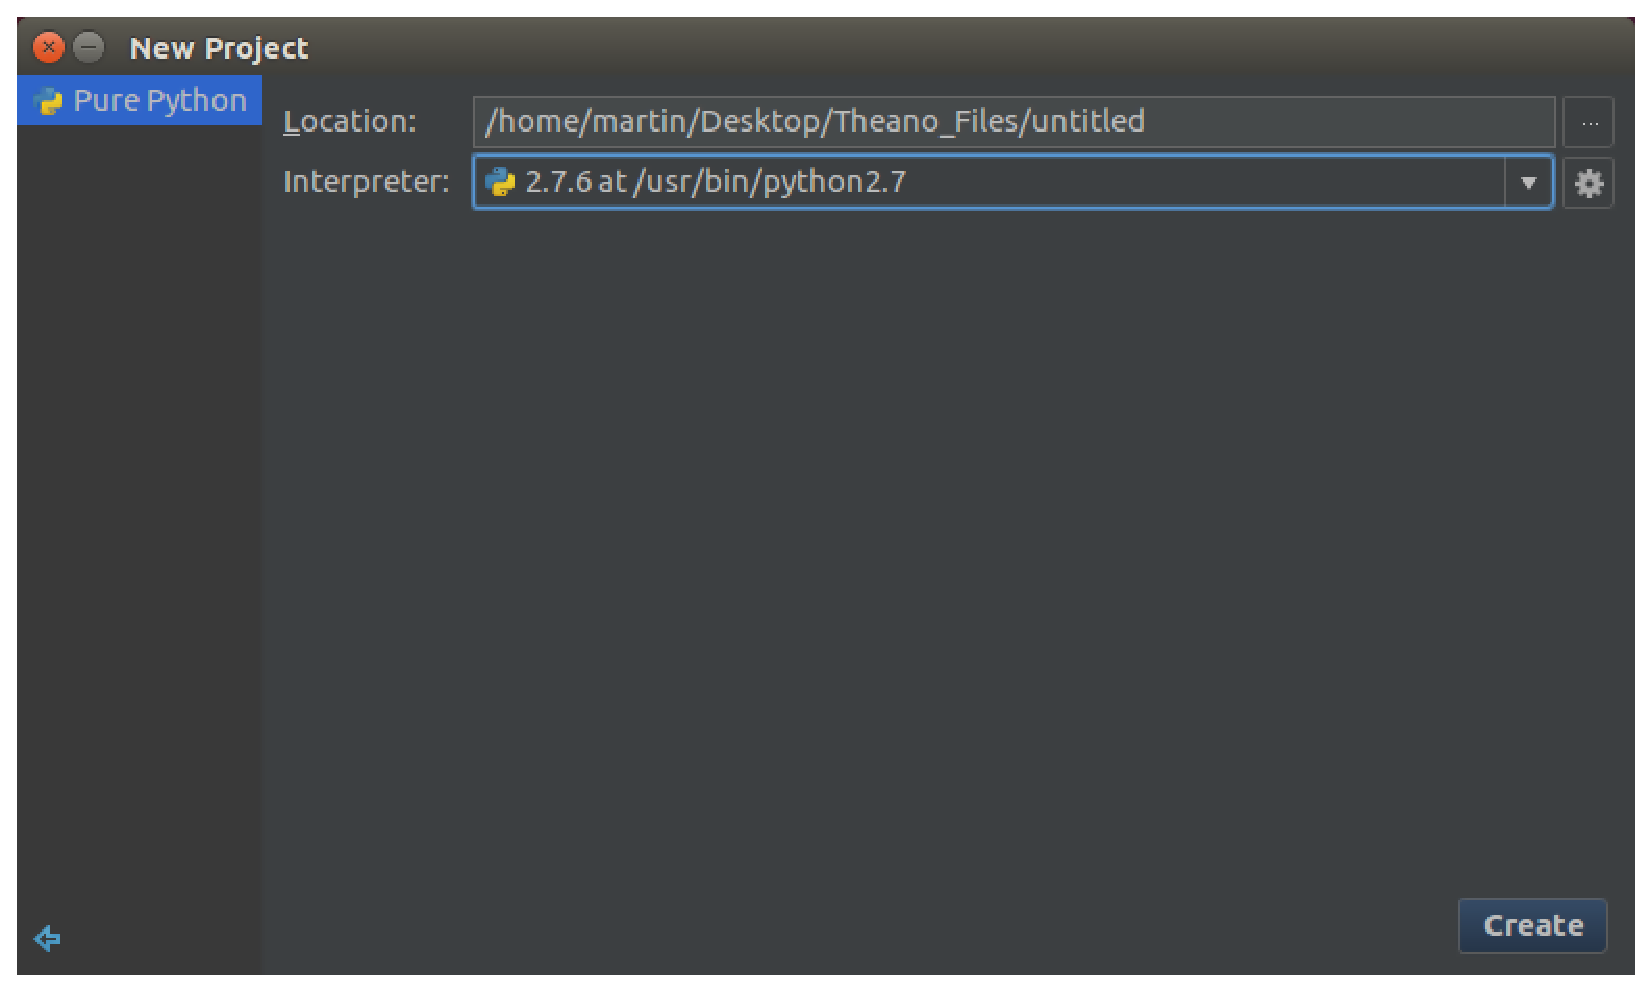
\includegraphics[width=3.5in, height=2.5in]{fig/3.eps}}
	\caption{Create New Project}
	\label{fig:3}
\end{figure}
\resume{enumerate}
  \item Now you need to set two things Location and Interpreter.
  \item Basically, location is the path that you are saving your files (Your folder).
  \item Interpreter needs to be set as python 2.7.
  \item Now press create bottom and by this time, you should be able to see Figure \ref{fig:4}.
\suspend{enumerate}
\begin{figure}[h]
	\centerline{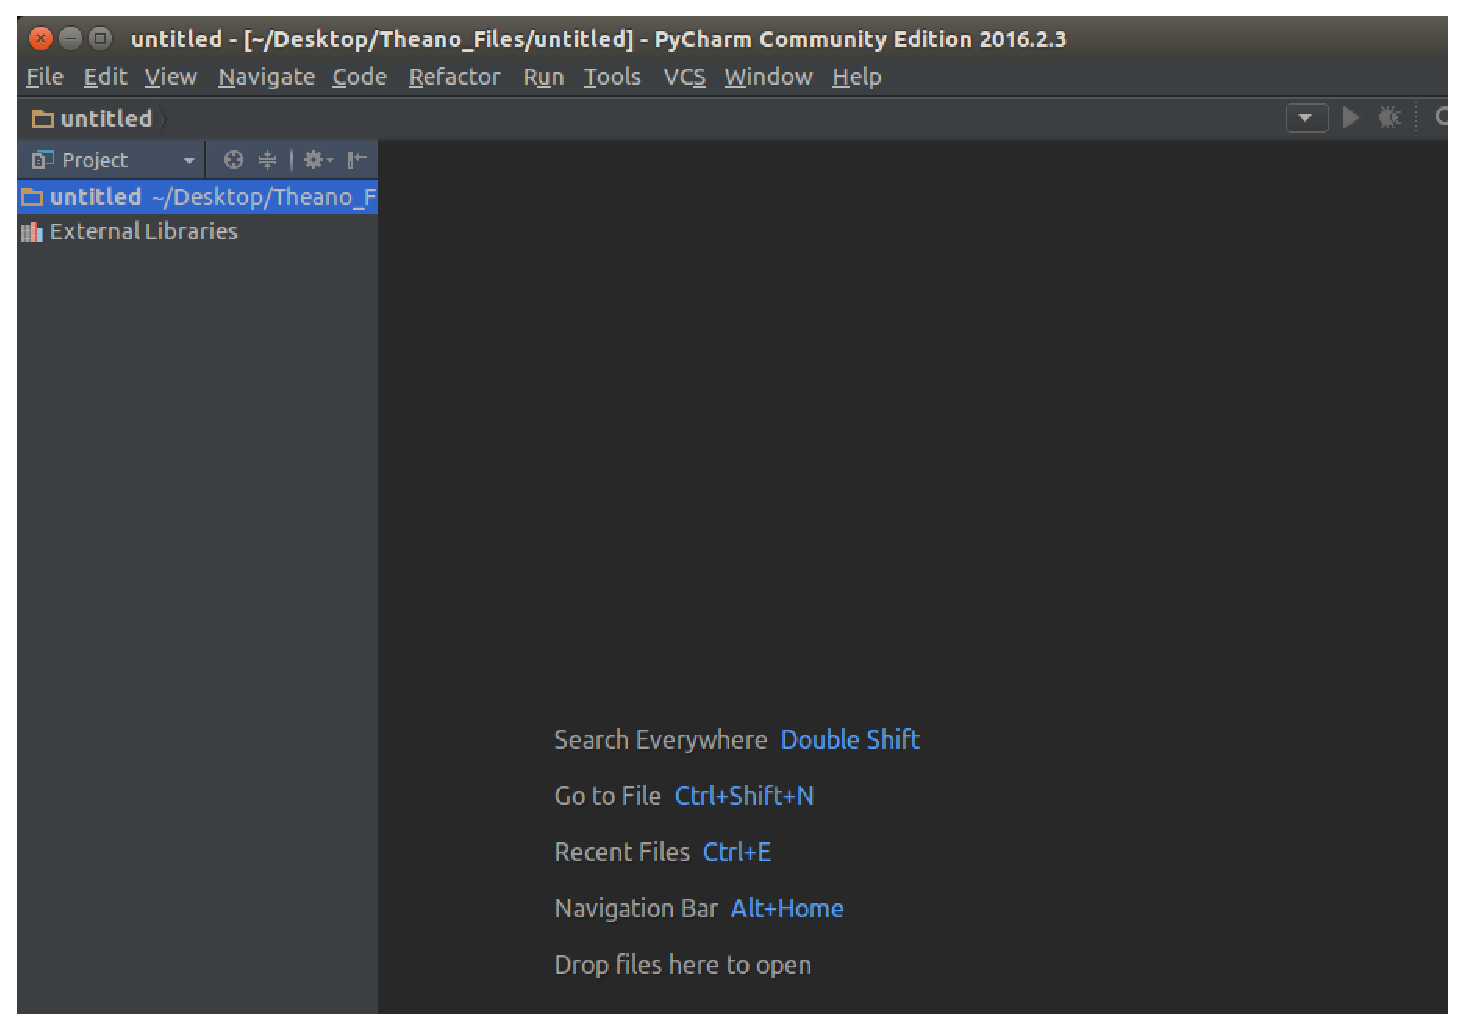
\includegraphics[width=3.5in, height=2.5in]{fig/4.eps}}
	\caption{Pycharm IDE Interface }
	\label{fig:4}
\end{figure}
\resume{enumerate}
  \item Go to the menu bar click on file.
  \item Click on New.
  \item Click on Pyhton File.
  \item Create the pyhton file and pick an arbitrary name.
  \item It will open up a new blank page that you can write your caffe program.
  \item Before start writing your code, you need to set the CUDA and Python environment.
  \item Now, you need to go to menu bar and this time choose Run and under Run.
  \item Choose Edit configuration, now you should be able to see the Figure \ref{fig:5}
\suspend{enumerate}
\begin{figure}[h]
	\centerline{\includegraphics[width=6.5in, height=3in]{fig/5.eps}}
	\caption{Edit Configuration}
	\label{fig:5}
\end{figure}
\resume{enumerate}
  \item Now you should be able to find Environment Variable.
  \item Click on the three dots icon.
  \item Now, you should be able to see the Figure \ref{fig:6}.
  \item This is the place we need to add our paths of CUDA and Python.
  \item There is a green plus icon.
  \item Click on it.
\suspend{enumerate}
\begin{figure}[ht]
	\centerline{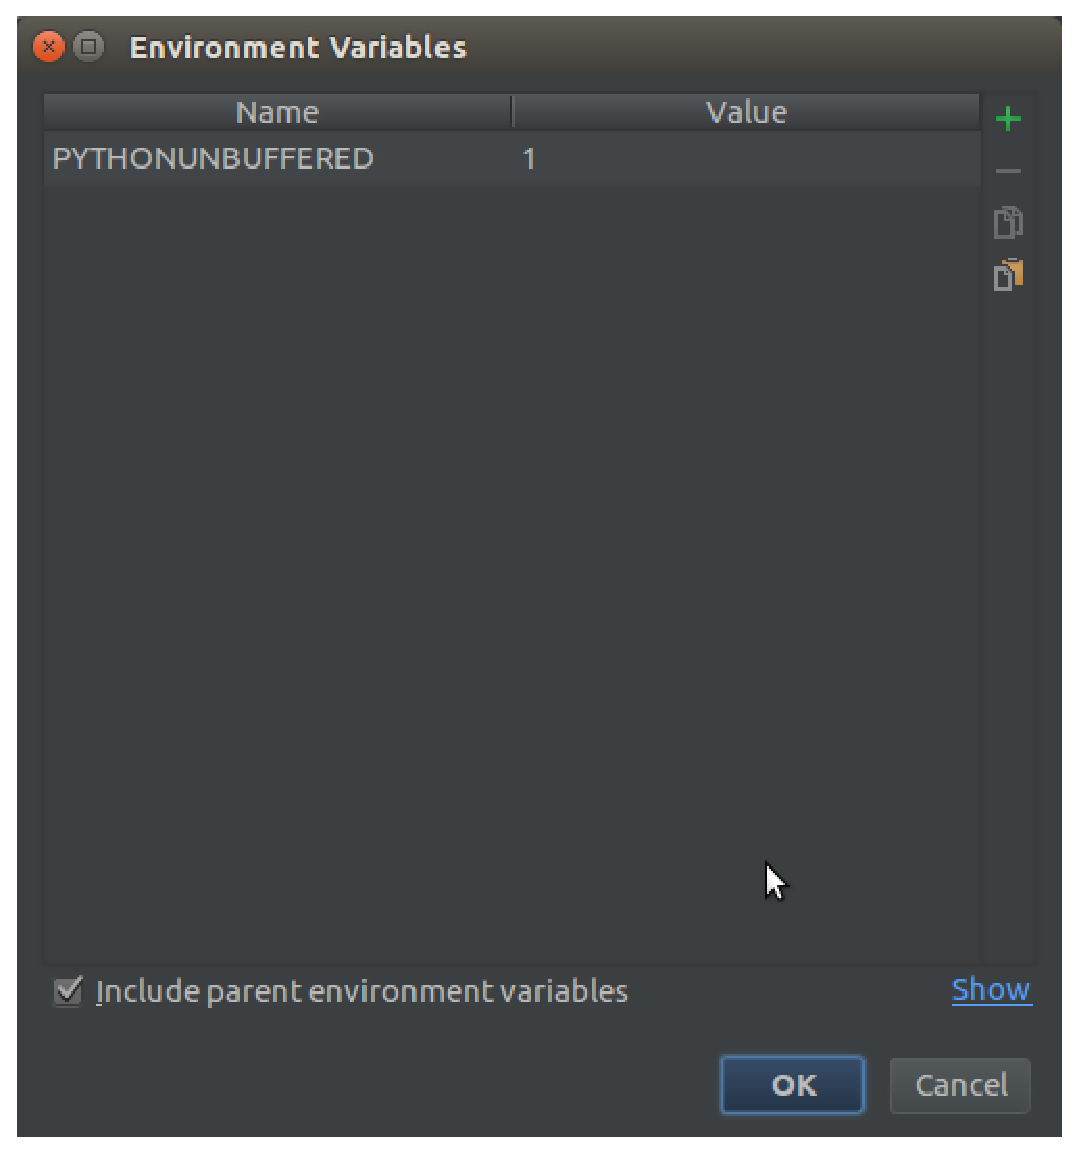
\includegraphics[width=3in, height=2in]{fig/6.eps}}
	\caption{Environment Variable}
	\label{fig:6}
\end{figure}
\resume{enumerate}
  \item There are two places we need to add our paths and name.
  \item In the Name box type the Following
  \item CAFFE\_ROOT
  \item In Value box type the Following
  \item /home/martin/caffe
  \item Click on the green plus icon again
  \item In the Name box type the Following
  \item LD\_LIBRARY\_PATH
  \item In Value box type the Following
  \item /usr/local/cuda/lib64
  \item Click on the green plus icon again
  \item In the Name box type the Following
  \item PYTHONPATH
  \item In Value box type the Following
  \item /home/martin/caffe/python
  \item Press OK and Finish.
  \item Now you should be able to import caffe.
  \item \textbf{Note: these setting needs to be done just once for each project you creating it for caffe. In other words now if you add another python file to this project under file and new you do not need to redo these settings.}
\end{enumerate}

\section{Theano}
\begin{enumerate}
  \item To use Theano software in Pycharm, you need to set the environments for CUDA and Python path.
  \item Open up VNC server and use your password to enter the Linux station.
  \item By this time you should be able to see the Ubuntu Desktop shown in Figure \ref{fig:1_1}.
\suspend{enumerate}
\begin{figure}[h]
	\centerline{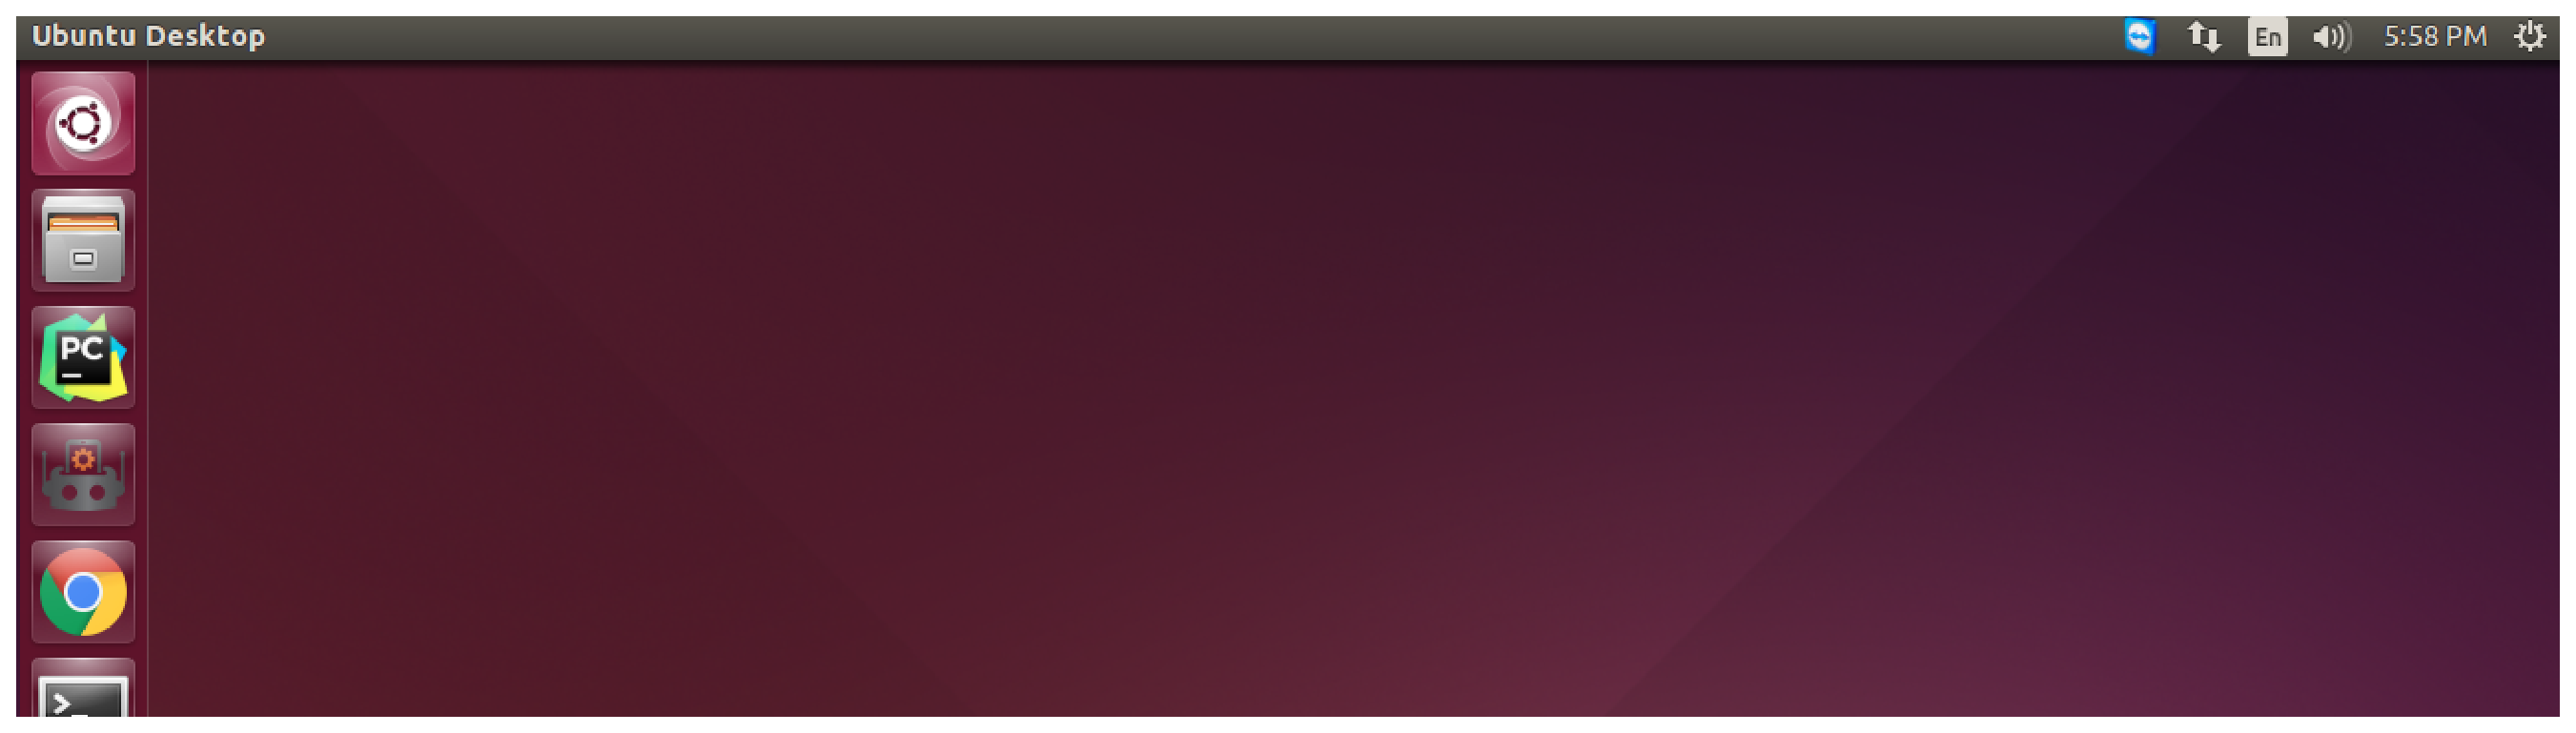
\includegraphics[width=6in, height=2in]{fig/1.eps}}
	\caption{Ubuntu Desktop-Theano}
	\label{fig:1_1}
\end{figure}
\resume{enumerate}
  \item On the top left corner of the Ubuntu Desktop, the first icon is search box under the search box is the folder icon.
  \item Click on it and go to your directory under your name and put a theano python file there call it test.py .
  \item On the top left corner of the Ubuntu Desktop again, the first icon is search box.
  \item Click on it and search the terminal.
  \item By this time you should be able to see the terminal and launch it by clicking on it.
  \item By this time, you should be able to see Figure \ref{fig:7}
  \item Now you need to use cd commend to change your directory in terminal.
  \item For example cd Desktop change your directory to Desktop.
  \item Change your directory by using cd command to your folder.
  \item now enter the following commands.
\suspend{enumerate}
\begin{figure}[ht]
	\centerline{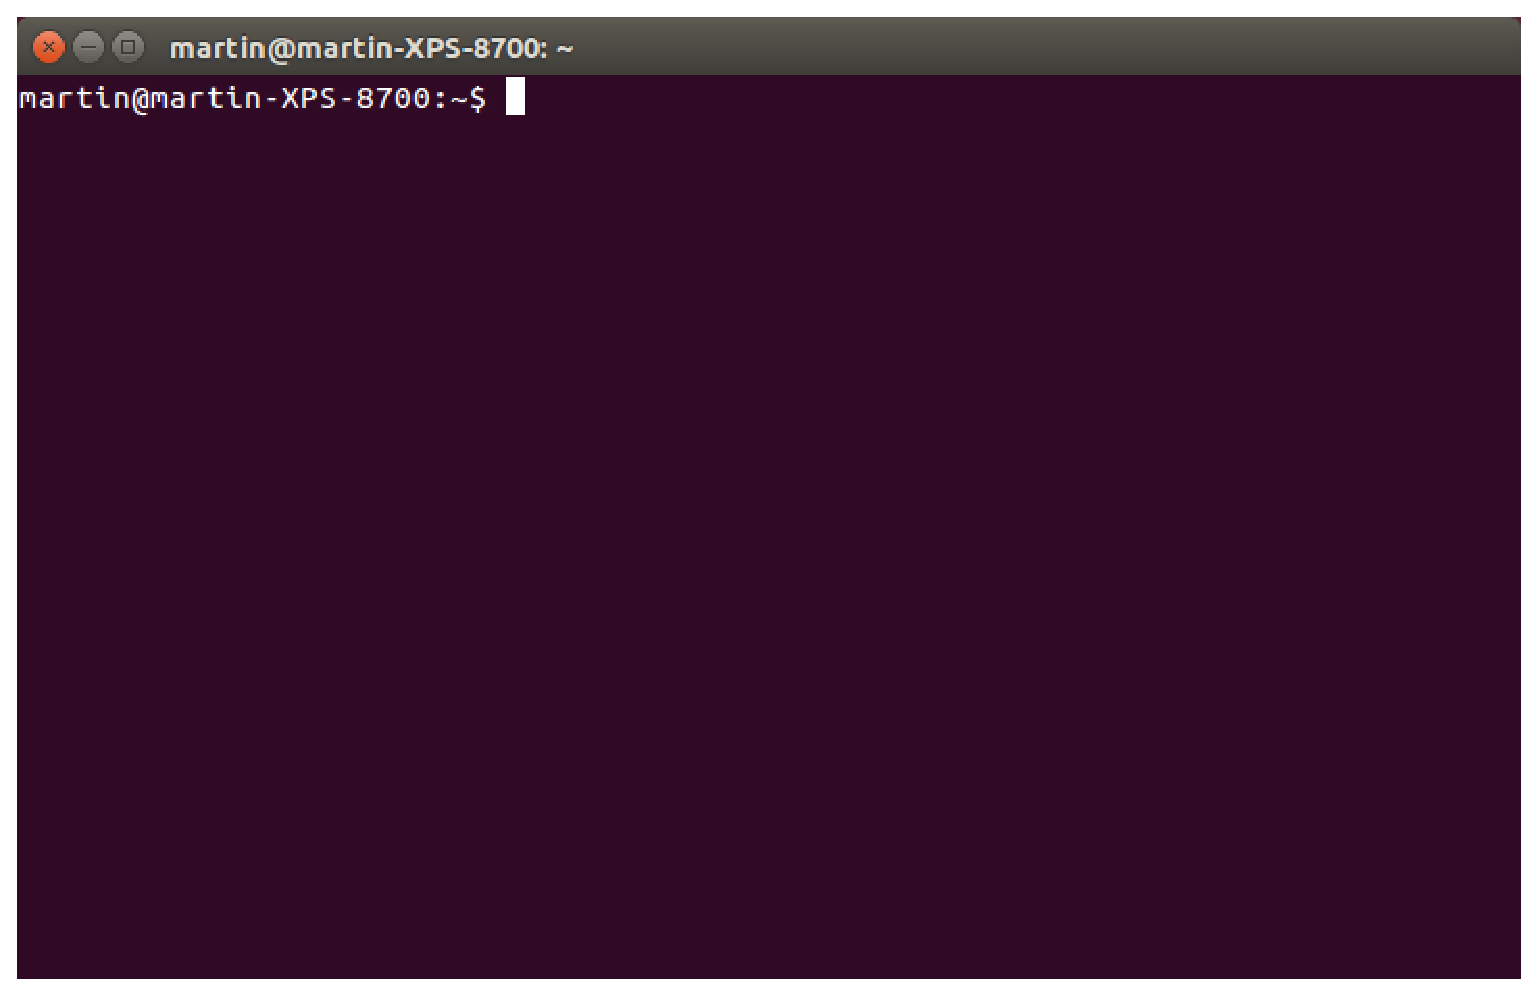
\includegraphics[width=4in, height=2.5in]{fig/7.eps}}
	\caption{Terminal}
	\label{fig:7}
\end{figure}
\begin{lstlisting}
    $ export LD_LIBRARY_PATH=/usr/local/cuda-7.5/lib64:$LD_LIBRARY_PATH

    $ export PATH=/usr/local/cuda-7.5/bin:$PATH

    $ pycharm-community test.py &
\end{lstlisting}

\resume{enumerate}
  \item Now pycharm automatically will open and you can run and test your code.
  \item Each you need to work with theano in pycharm you need to start over the process from the first step.
\end{enumerate}
\newpage
\section{Tesnsorflow}
\begin{enumerate}
  \item To use Tensorflow software in Pycharm, you need to set the environments for CUDA and Python path.
  \item Open up VNC server and use your password to enter the Linux station.
  \item By this time you should be able to see the Ubuntu Desktop shown in Figure \ref{fig:1_2}.
\suspend{enumerate}
\begin{figure}[h]
	\centerline{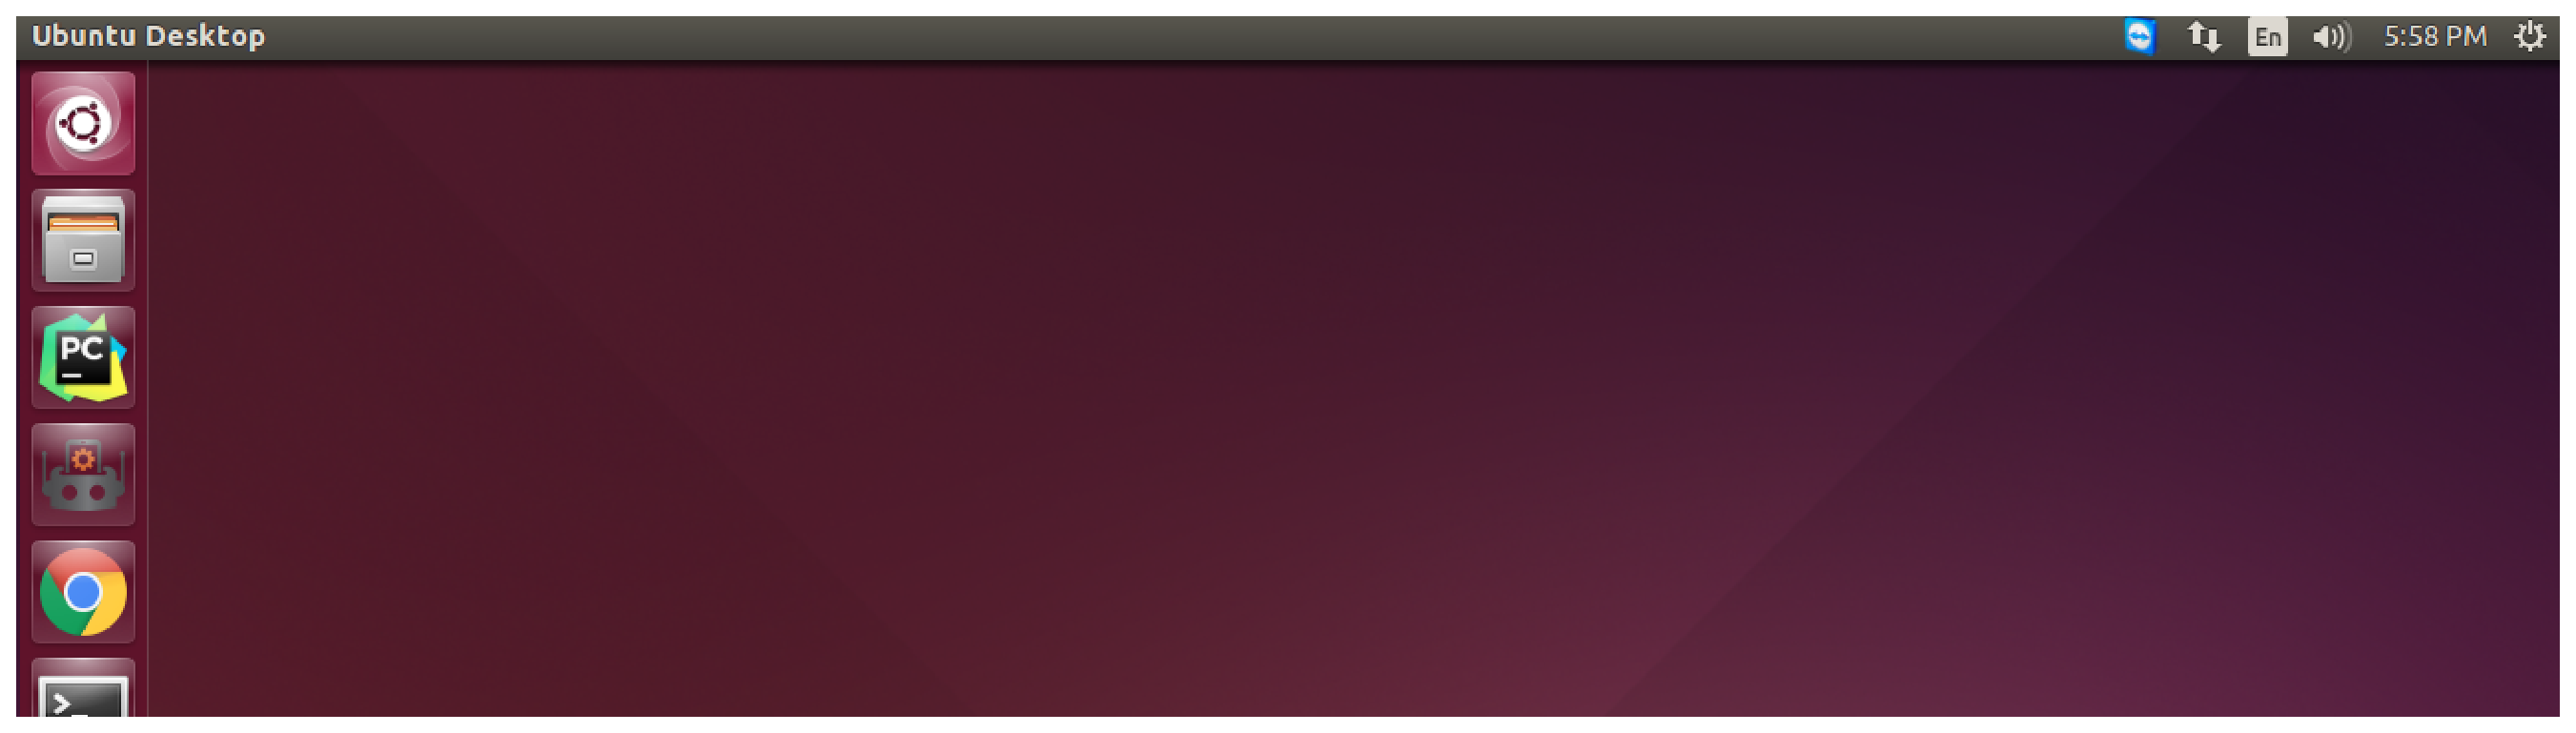
\includegraphics[width=6in, height=1.6in]{fig/1.eps}}
	\caption{Ubuntu Desktop-Tesnsorflow}
	\label{fig:1_2}
\end{figure}
\resume{enumerate}
  \item On the top left corner of the Ubuntu Desktop, the first icon is search box.
  \item Click on it and search the word pycharm.
  \item By this time you should be able to see the pycharm IDE and launch it by clicking on it.
  \item By this time, you should be able to see Figure \ref{fig:2_1}
\suspend{enumerate}
\begin{figure}[h]
	\centerline{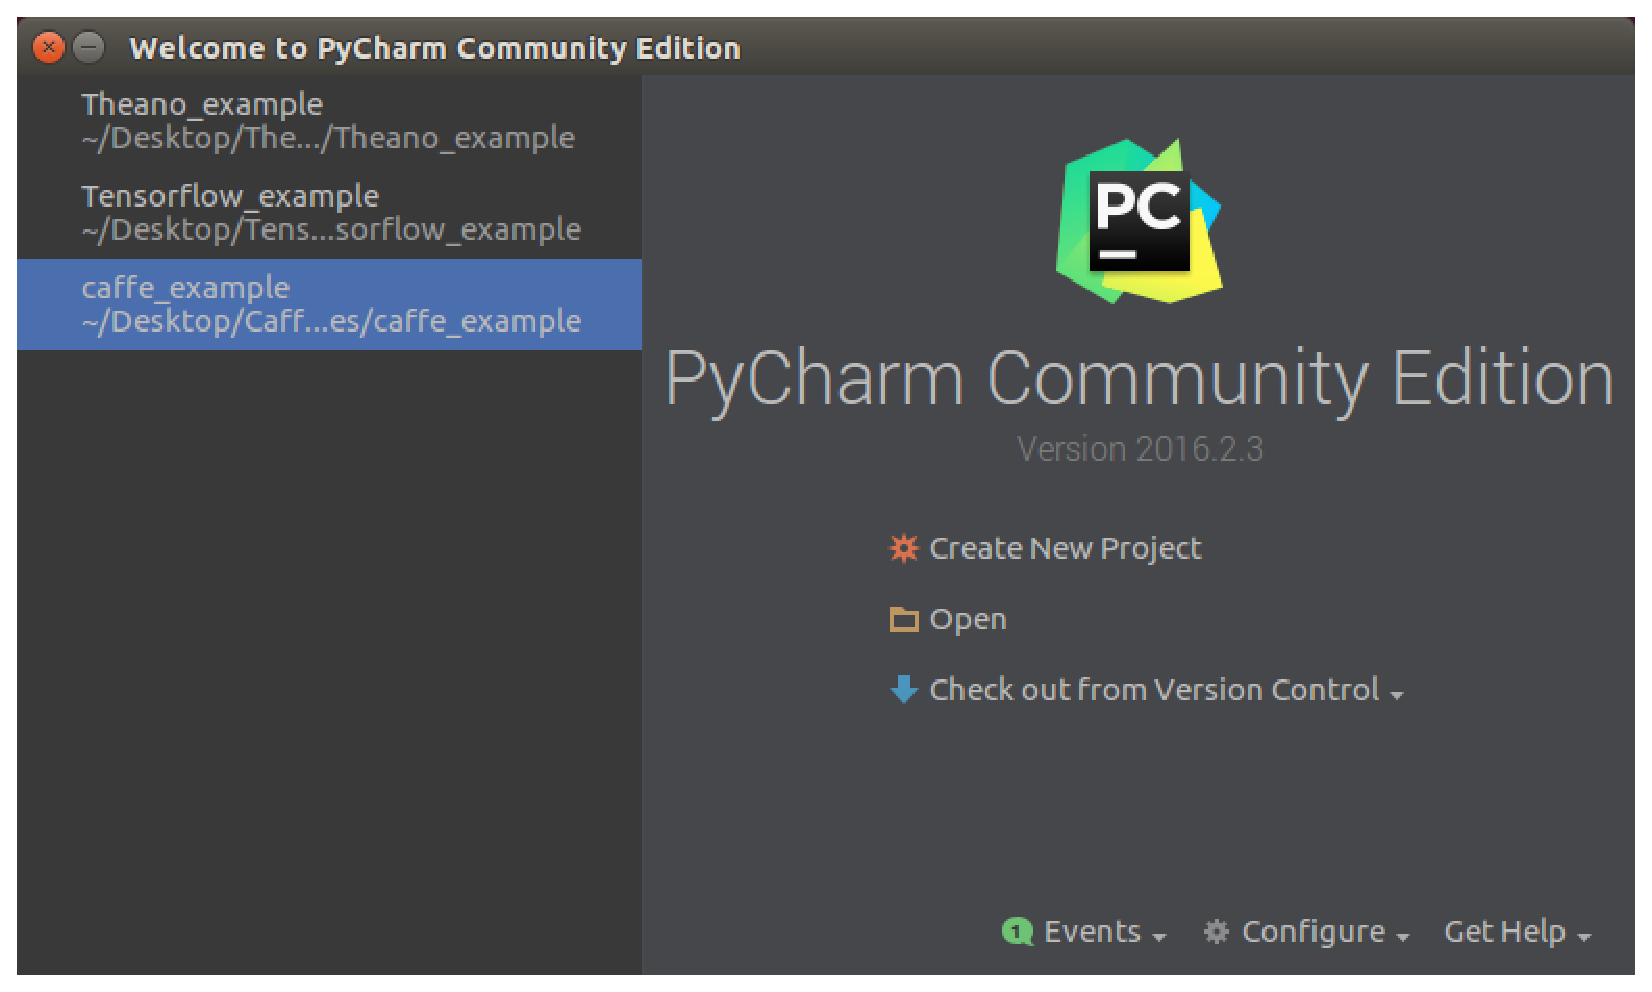
\includegraphics[width=3.5in, height=2.3in]{fig/2.eps}}
	\caption{Pycharm IDE-Tensorflow}
	\label{fig:2_1}
\end{figure}
\resume{enumerate}
  \item Now, we need to create a project, click on create new project icon.
  \item It opens up a new window shown in Figure \ref{fig:3_1}.
\suspend{enumerate}
\begin{figure}[h]
	\centerline{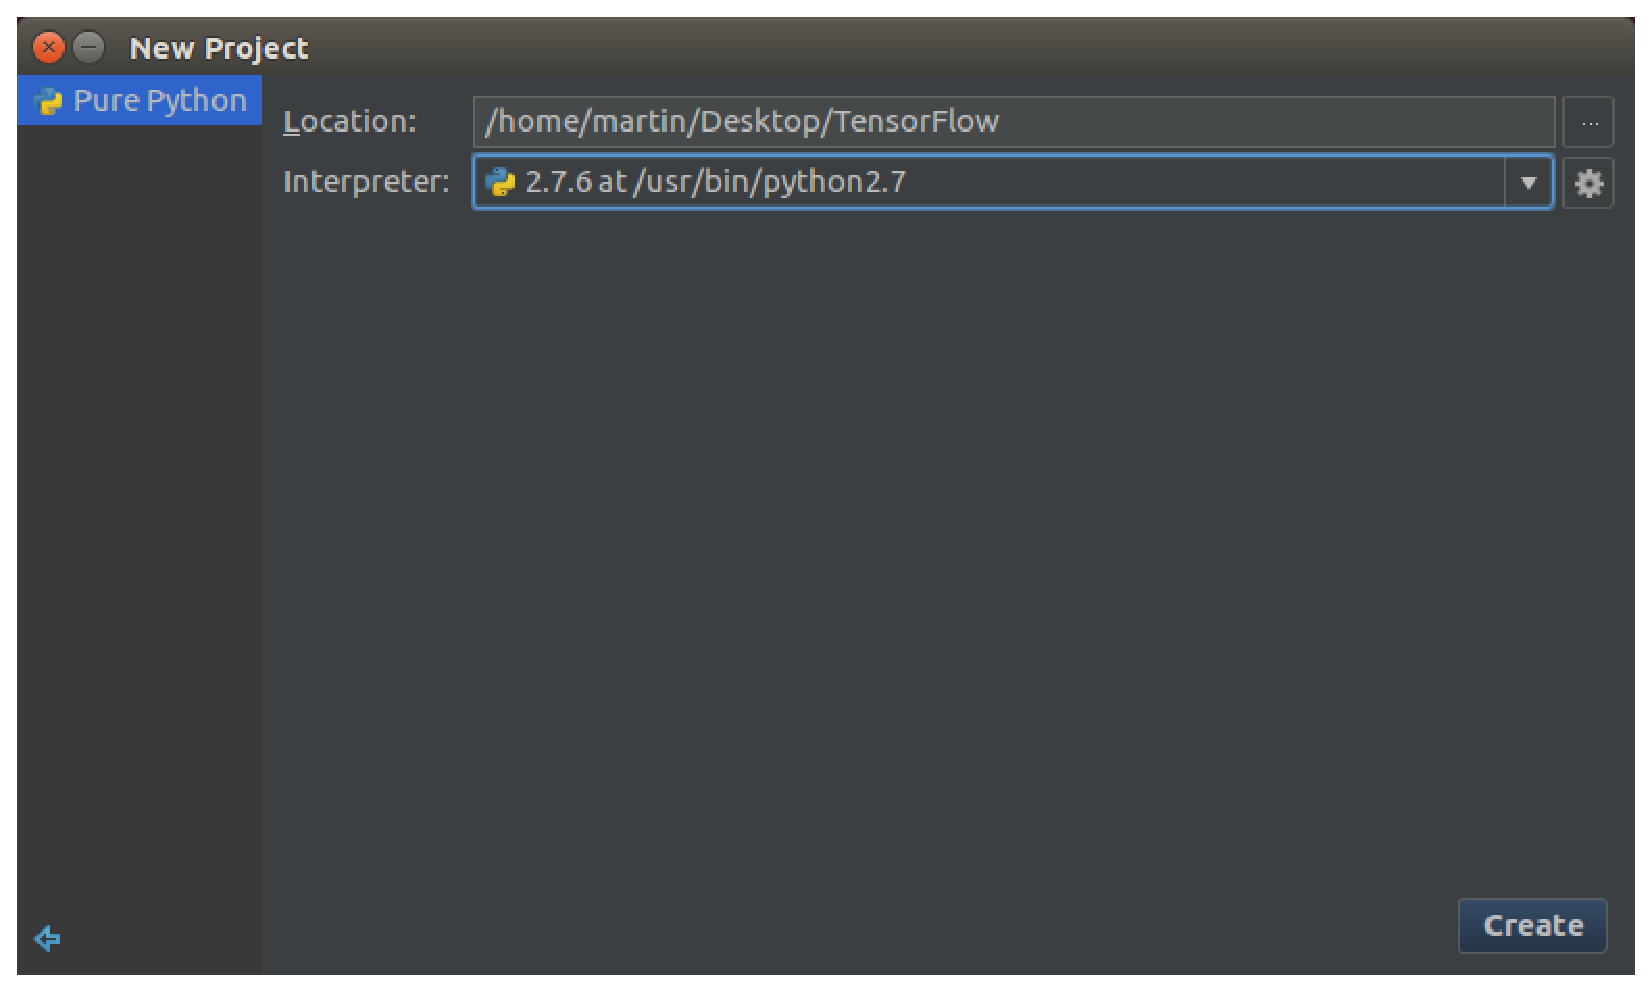
\includegraphics[width=3.5in, height=2.3in]{fig/8.eps}}
	\caption{Create New Project -Tensorflow}
	\label{fig:3_1}
\end{figure}
\resume{enumerate}
  \item Now you need to set two things Location and Interpreter.
  \item Basically, location is the path that you are saving your files (Your folder).
  \item Interpreter needs to be set as python 2.7.
  \item Now press the gear box in front of the Interpreter.
  \item A small window will pop up and click on Create VirtualEnv.
  \item Now you should be able to see the Figure \ref{fig:10}
\suspend{enumerate}
\begin{figure}[h]
	\centerline{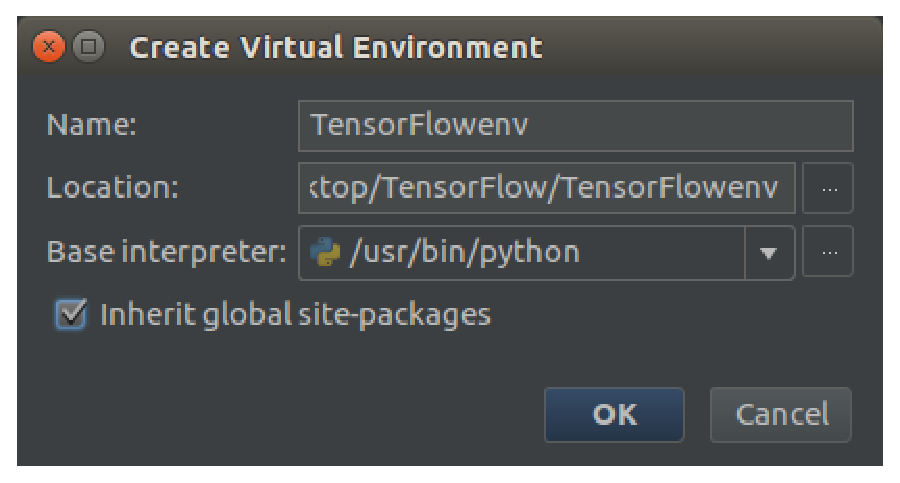
\includegraphics[width=3.5in, height=2in]{fig/10.eps}}
	\caption{Create Virtual Environment}
	\label{fig:10}
\end{figure}
\resume{enumerate}
  \item Choose name as TensorFlowenv
  \item Basically, location is the path that you are saving your files (Your folder).
  \item Check the inherit global site-packages.
  \item Click on the 3 dots in front of Base interpreter.
  \item It will open up a directories that includes all interpreters shown in Figure \ref{fig:9}.
  \item Click on python and click OK the press Create.
\suspend{enumerate}
\begin{figure}[h]
	\centerline{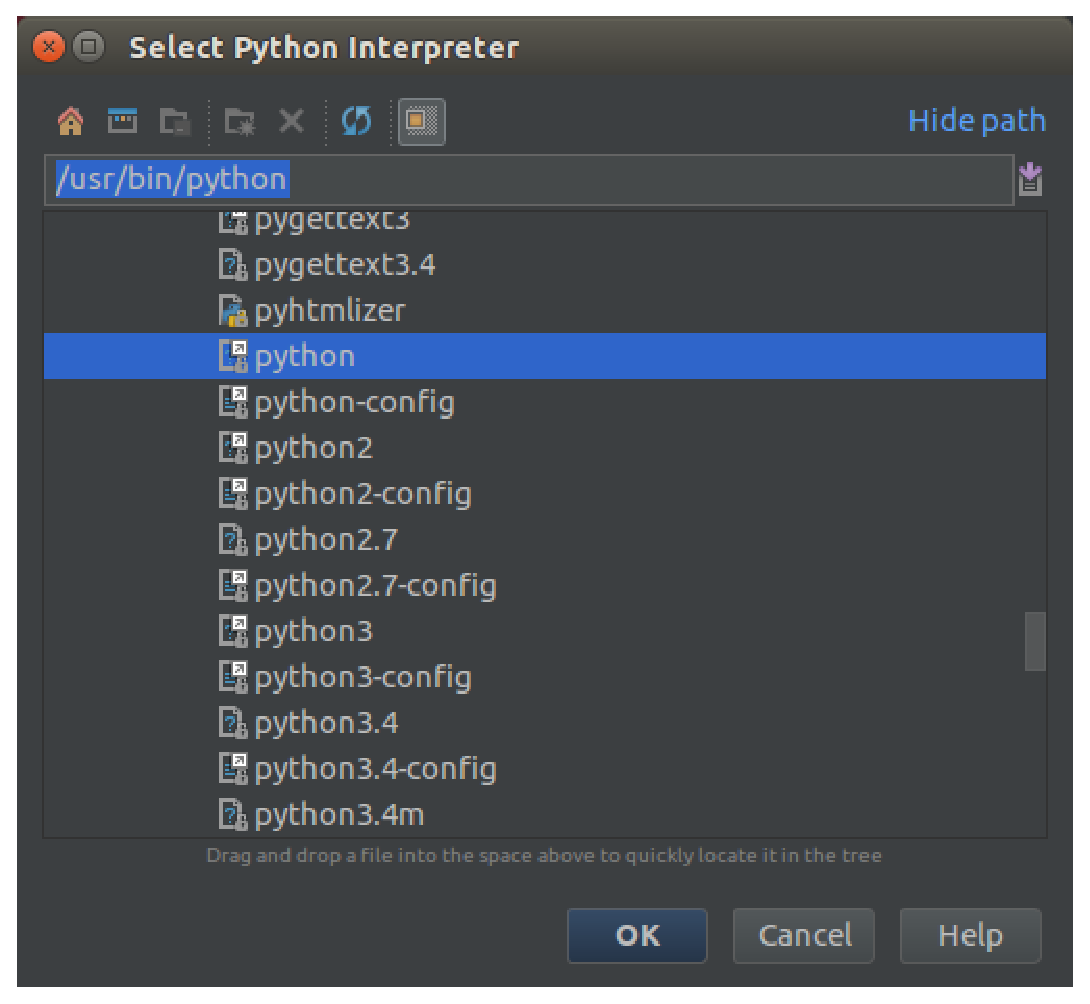
\includegraphics[width=4in, height=2.4in]{fig/9.eps}}
	\caption{Base Interpreter}
	\label{fig:9}
\end{figure}
\resume{enumerate}
  \item Now, you should be able to see Figure \ref{fig:11}.
\suspend{enumerate}
\begin{figure}[h]
	\centerline{\includegraphics[width=3.5in, height=2.4in]{fig/11.eps}}
	\caption{Pycharm IDE Interface Tensorflow }
	\label{fig:11}
\end{figure}
\resume{enumerate}
  \item Go to the menu bar click on file.
  \item Click on New.
  \item Click on Pyhton File.
  \item Create the pyhton file and pick an arbitrary name.
  \item It will open up a new blank page that you can write your Tensorflow program.
  \item Before start writing your code, you need to set the CUDA and Python environment.
  \item Now, you need to go to menu bar and this time choose Run and under Run.
  \item Choose Edit configuration, now you should be able to see the Figure \ref{fig:5_1}
\suspend{enumerate}
\begin{figure}[h]
	\centerline{\includegraphics[width=6.5in, height=3in]{fig/5.eps}}
	\caption{Edit Configuration TensorFlow}
	\label{fig:5_1}
\end{figure}
\resume{enumerate}
  \item Now you should be able to find Environment Variable.
  \item Click on the three dots icon.
  \item Now, you should be able to see the Figure \ref{fig:6_1}.
  \item This is the place we need to add our paths of CUDA and Python.
  \item There is a green plus icon.
  \item Click on it.
\suspend{enumerate}
\begin{figure}[ht]
	\centerline{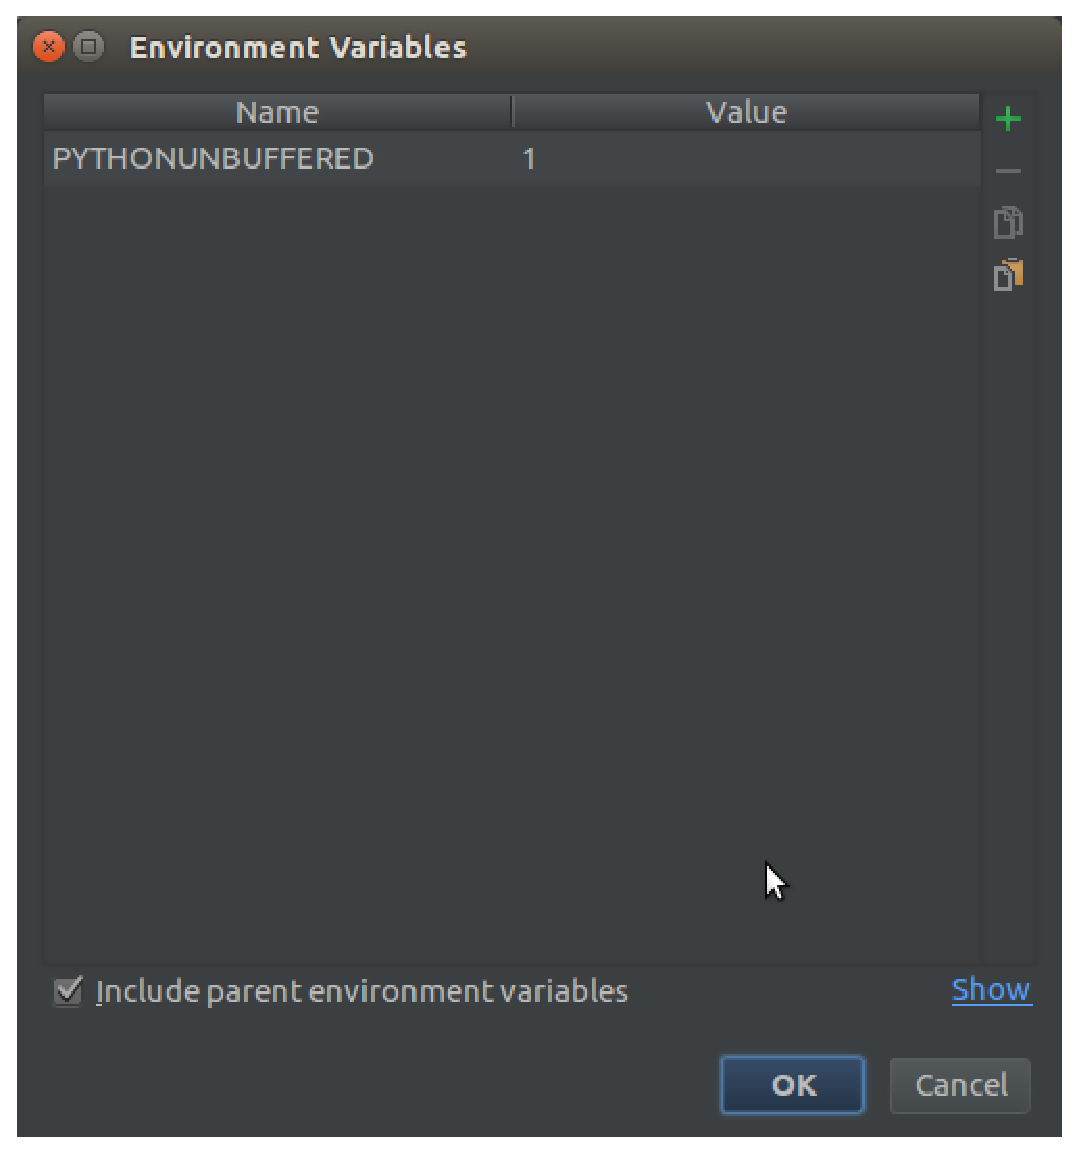
\includegraphics[width=3in, height=2in]{fig/6.eps}}
	\caption{Environment Variable Tensorflow}
	\label{fig:6_1}
\end{figure}
\resume{enumerate}
  \item There are two places we need to add our paths and name.
  \item In the Name box type the Following
  \item PATH
  \item In Value box type the Following
  \item /usr/local/cuda-7.5/bin
  \item Click on the green plus icon again
  \item In the Name box type the Following
  \item LD\_LIBRARY\_PATH
  \item In Value box type the Following
  \item /usr/local/cuda/lib64
  \item Press OK and Finish.
  \item Now you should be able to import Tensorflow.
  \item \textbf{Note: these setting needs to be done just once for each project you creating it for Tesnsorflow. In other words now if you add another python file to this project under file and new you do not need to redo these settings.}
\end{enumerate}





\end{document}
